%!TEX program = xelatex

\documentclass[a4paper, openany, oneside]{memoir}
\usepackage[no-math]{fontspec}
\usepackage{pgfplots}
\pgfplotsset{compat=newest}
\usepackage{commath}
\usepackage{mathtools}
\usepackage{amssymb}
\usepackage{amsthm}
\usepackage{booktabs}
\usepackage{mathtools}
\usepackage{xcolor}
\usepackage[separate-uncertainty=true, per-mode=symbol]{siunitx}
\usepackage[noabbrev, capitalize]{cleveref}
\usepackage{listings}
\usepackage[american inductor, european resistor]{circuitikz}
\usepackage{amsmath}
\usepackage{amsfonts}
\usepackage{ifxetex}
\usepackage[dutch,english]{babel}
\usepackage[backend=bibtexu,texencoding=utf8,bibencoding=utf8,style=ieee,sortlocale=en_GB,language=auto]{biblatex}
\usepackage[strict,autostyle]{csquotes}
\usepackage{parskip}
\usepackage{import}
\usepackage{standalone}
\usepackage{hyperref}
%\usepackage[toc,title,titletoc]{appendix}

\ifxetex{} % Fonts laden in het geval dat je met Xetex compiled
    \usepackage{fontspec}
    \defaultfontfeatures{Ligatures=TeX} % To support LaTeX quoting style
    \setromanfont{Palatino Linotype} % Tover ergens in Font mapje in root.
    \setmonofont{Source Code Pro}
\else % Terug val in standaard pdflatex tool chain. Geen ondersteuning voor OTT fonts
    \usepackage[T1]{fontenc}
    \usepackage[utf8]{inputenc}
\fi
\newcommand{\references}[1]{\begin{flushright}{#1}\end{flushright}}
\renewcommand{\vec}[1]{\boldsymbol{\mathbf{#1}}}
\newcommand{\uvec}[1]{\boldsymbol{\hat{\vec{#1}}}}
\newcommand{\mat}[1]{\boldsymbol{\mathbf{#1}}}
\newcommand{\fasor}[1]{\boldsymbol{\tilde{\vec{#1}}}}
\newcommand{\cmplx}[0]{\mathrm{j}}
\renewcommand{\Re}[0]{\operatorname{Re}}
\newcommand{\Cov}{\operatorname{Cov}}
\newcommand{\Var}{\operatorname{Var}}
\newcommand{\proj}{\operatorname{proj}}
\newcommand{\Perp}{\operatorname{perp}}
\newcommand{\col}{\operatorname{col}}
\newcommand{\rect}{\operatorname{rect}}
\newcommand{\sinc}{\operatorname{sinc}}
\newcommand{\IT}{\operatorname{IT}}
\newcommand{\F}{\mathcal{F}}

\newtheorem{definition}{Definition}
\newtheorem{theorem}{Theorem}


\DeclareSIUnit{\voltampere}{VA} %apparent power
\DeclareSIUnit{\pii}{\ensuremath{\pi}}

\hypersetup{%setup hyperlinks
    colorlinks,
    citecolor=black,
    filecolor=black,
    linkcolor=black,
    urlcolor=black
}

% Example boxes
\usepackage{fancybox}
\usepackage{framed}
\usepackage{adjustbox}
\newenvironment{simpages}%
{\AtBeginEnvironment{itemize}{\parskip=0pt\parsep=0pt\partopsep=0pt}
\def\FrameCommand{\fboxsep=.5\FrameSep\shadowbox}\MakeFramed{\FrameRestore}}%
{\endMakeFramed}

% Impulse train
\DeclareFontFamily{U}{wncy}{}
\DeclareFontShape{U}{wncy}{m}{n}{<->wncyr10}{}
\DeclareSymbolFont{mcy}{U}{wncy}{m}{n}
\DeclareMathSymbol{\Sha}{\mathord}{mcy}{"58}
\addbibresource{../../../../includes/bibliography.bib}

\begin{document}
\section{Introduction}
This chapter is an introduction to concepts which will be key in the design of our system.
% \section{Concept}
\section{Uniform sampling}
As described by the system overview in \cref{cha:overview}, the first step in high-performance spectrum sensing consists of sampling the signal. Conventional methods sample at an uniform sampling rate, which means that the time between the sample moments is constant. Uniform sampling is illustrated in \cref{tkz:uniform}. Here blocks represent samples such that subsequent rectangles are subsequent samples.

\begin{figure}[H]
\centering
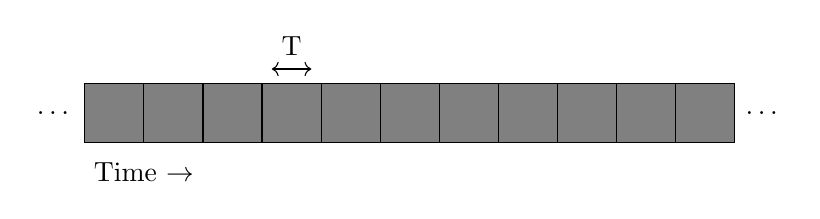
\begin{tikzpicture}[scale=0.75]

\draw [fill=gray]  (-2,0) rectangle (-1,-1);
\draw [fill=gray]  (-1,0) rectangle (0,-1);
\draw [fill=gray]  (0,0) rectangle (1,-1);
\draw [fill=gray]  (1,0) rectangle (2,-1);
\draw [fill=gray]  (2,0) rectangle (3,-1);
\draw [fill=gray]  (3,0) rectangle (4,-1);
\draw [fill=gray]  (4,0) rectangle (5,-1);
\draw [fill=gray]  (5,0) rectangle (6,-1);
\draw [fill=gray]  (6,0) rectangle (7,-1);
\draw [fill=gray]  (7,0) rectangle (8,-1);
\draw [fill=gray]  (8,0) rectangle (9,-1);

\node (v1) at (-2.5,-.5) {};
\node (v2) at (9.5,-.5) {};
\draw  (v1) node {\dots} ;
\draw  (v2) node {\dots} ;

\node (v3) at (1,.25) {};
\node (v4) at (2,.25) {};
\draw  [<->] (v3) edge (v4);

\node (v5) at (1.5,.5) {};
\draw  (v5) node[yshift=0.1cm] {T} ;
\draw (-1,-1.5) node {Time $\rightarrow$};
\end{tikzpicture}
\caption{Uniform sampling with sampling period $T$}\label{tkz:uniform}
\end{figure}

\section{Non-uniform sampling}

When one desires to ensure full reconstruction of an uniformly sampled signal, one needs to sample this signal at least at the Nyquist frequency. However, we are not necessarily interested in full recovery of the signal, since we only need to detect which frequencies of the signal are occupied by signals distinct from noise. In our sampling methods, we aim to not restrict ourselves to uniform sampling, and try to exploit non-uniform sampling. This allows for methods which sample the signal in a more efficient way. Since we aim to solely obtain the power spectral density of the signal, it turns out that by non-uniform sampling, we can still do this. Non-uniform sampling is illustrated in \cref{tkz:nonuniform}. This figure is similar to \cref{tkz:uniform}, but some blocks are left white. Only the grey blocks represent sample moments of the non-uniform sampler.

\begin{figure}[H]
\centering
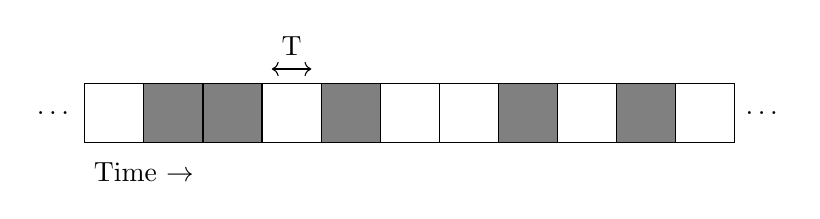
\begin{tikzpicture}[scale=0.75]

\draw  (-2,0) rectangle (-1,-1);
\draw [fill=gray]  (-1,0) rectangle (0,-1);
\draw [fill=gray]  (0,0) rectangle (1,-1);
\draw  (1,0) rectangle (2,-1);
\draw [fill=gray] (2,0) rectangle (3,-1);
\draw  (3,0) rectangle (4,-1);
\draw  (4,0) rectangle (5,-1);
\draw [fill=gray]  (5,0) rectangle (6,-1);
\draw  (6,0) rectangle (7,-1);
\draw  [fill=gray] (7,0) rectangle (8,-1);
\draw  (8,0) rectangle (9,-1);

\node (v1) at (-2.5,-.5) {};
\node (v2) at (9.5,-.5) {};
\draw  (v1) node {\dots} ;
\draw  (v2) node {\dots} ;

\node (v3) at (1,.25) {};
\node (v4) at (2,.25) {};
\draw  [<->] (v3) edge (v4);

\node (v5) at (1.5,.5) {};
\draw  (v5) node[yshift=0.1cm] {T} ;
\draw (-1,-1.5) node {Time $\rightarrow$};
\end{tikzpicture}
\caption{Non-uniform sampling with sampling period $T$. Grey blocks represent sample moments of the non-uniform sampler.}\label{tkz:nonuniform}
\end{figure}

\section{Multi-coset sampling}
Non-uniform sampling, however, is not trivial to implement. To perform non-uniform sampling, we introduce a concept called multi-coset sampling. Multi-coset sampling is the name for a set of sampling methods that use multiple samplers which sample the same signal. These samplers are also called cosets. From now on, we will use these two terms interchangeably. Multi-coset sampling is illustrated in \cref{tkz:multicoset}. Here the $x$ represents the input signal, the switches represent a sample operation and $y_i$ represent the outputs of the different cosets. In \cref{cha:reconstruction}, we will deduce criteria that will further specify the samplers. Afterwards, in \cref{cha:sampling_methods}, we will reconsider non-uniform sampling to optimise performance.

\begin{figure}
\centering
\begin{tikzpicture}
\draw  (-2.5,2) rectangle (-1.5,1) node[pos=.5]{$x$};
\draw  (-1.5,1.5) -- (0.5,1.5);
\draw  (-0.5,3) -- (0.5,3);
\draw (-0.5,3) -- (-0.5,-0.5);

\node at (2.5,-.91) {\vdots};
\node at (0.75,-.91) {\vdots};
\node at (-0.5,-.91) {\vdots};

\draw (-0.5,-1.5) -- (-0.5,-2);
\draw  (1,3) -- (2,3);
\draw  (1,1.5) -- (2,1.5);
\draw  (1,0) -- (2,0);
\draw  (1,-2) -- (2,-2);
\draw (-0.5,0) -- (0.5,0);
\draw (-0.5,-2) -- (0.5,-2);
\draw[ very thick](0.5,3)-- +(30:0.46);
\draw[ very thick](0.5,1.5)-- +(30:0.46);
\draw[ very thick](0.5,0)-- +(30:0.46);
\draw[ very thick](0.5,-2)-- +(30:0.46);
\draw  (3,2) rectangle (2,1) node[pos=.5]{$y_2$};
\draw  (3,0.5) rectangle (2,-0.5) node[pos=.5]{$y_3$};
\draw  (3,-1.5) rectangle (2,-2.5) node[pos=.5]{$y_M$};
\draw  (3,3.5) rectangle (2,2.5) node[pos=.5]{$y_1$};
\end{tikzpicture}
\caption{Conceptual schematic representation of multi-coset sampling with $M$ cosets}\label{tkz:multicoset}
\end{figure}

\end{document}

